\documentclass{beamer}
\usetheme{Rochester}
\addtobeamertemplate{navigation symbols}{}{ \hspace{1em}    \usebeamerfont{footline}%
	\insertframenumber / \inserttotalframenumber }
\begin{document}
	\title{Efficient and Scalable Bipartite Matching through Fast Beta Linkage (fabl)}
	%\subtitle{Using Beamer}
	\author{Brian Kundinger, Jerome Reiter, Rebecca Steorts}
	\institute{Duke University}
	\date{\today}
	
%	\AtBeginSection[]{
%		\begin{frame}
%			\vfill
%			\centering
%			\begin{beamercolorbox}[sep=8pt,center,shadow=true,rounded=true]{title}
%				\usebeamerfont{title}\insertsectionhead\par%
%			\end{beamercolorbox}
%			\vfill
%		\end{frame}
%	}

\AtBeginSection[]
{
	\begin{frame}
		\frametitle{Table of Contents}
		\tableofcontents[currentsection]
	\end{frame}
}
	
	\begin{frame}
		\titlepage
	\end{frame}

%	\begin{frame}
%	\frametitle{Outline}
%	\tableofcontents
%	\end{frame}

\section{Introduction to Record Linkage}

	\begin{frame}{What is Record Linkage?}
	\begin{enumerate}
		\item Record linkage is the task of identifying duplicate records over noisy datasets.
		
		\item Easy with unique identifiers, difficult when faced with errors
		
		\item Far ranging applications in business, public health, and human rights
	\end{enumerate}
	\end{frame}


\begin{frame}{Record Linkage in Practice}
	\begin{columns}
		\begin{column}{0.48\textwidth}
			\includegraphics<1->[width = \textwidth, height = 1.2\textwidth ]{ted_article2.png}
			
		\end{column}
		\begin{column}{0.48\textwidth}
			\includegraphics<2->[width = \textwidth, height = 1.2\textwidth ]{dnc_header.png}
		\end{column}
	\end{columns}
\end{frame}

	\begin{frame}{Linkage for Downstream Analysis}
	\includegraphics<1>[width = \textwidth, height = .7\textwidth ]{datasets.png}
	\includegraphics<2>[width = \textwidth, height = .7\textwidth ]{datasets_linked.png}

\end{frame}

	\begin{frame}{Linkage through Comparison Vectors}
		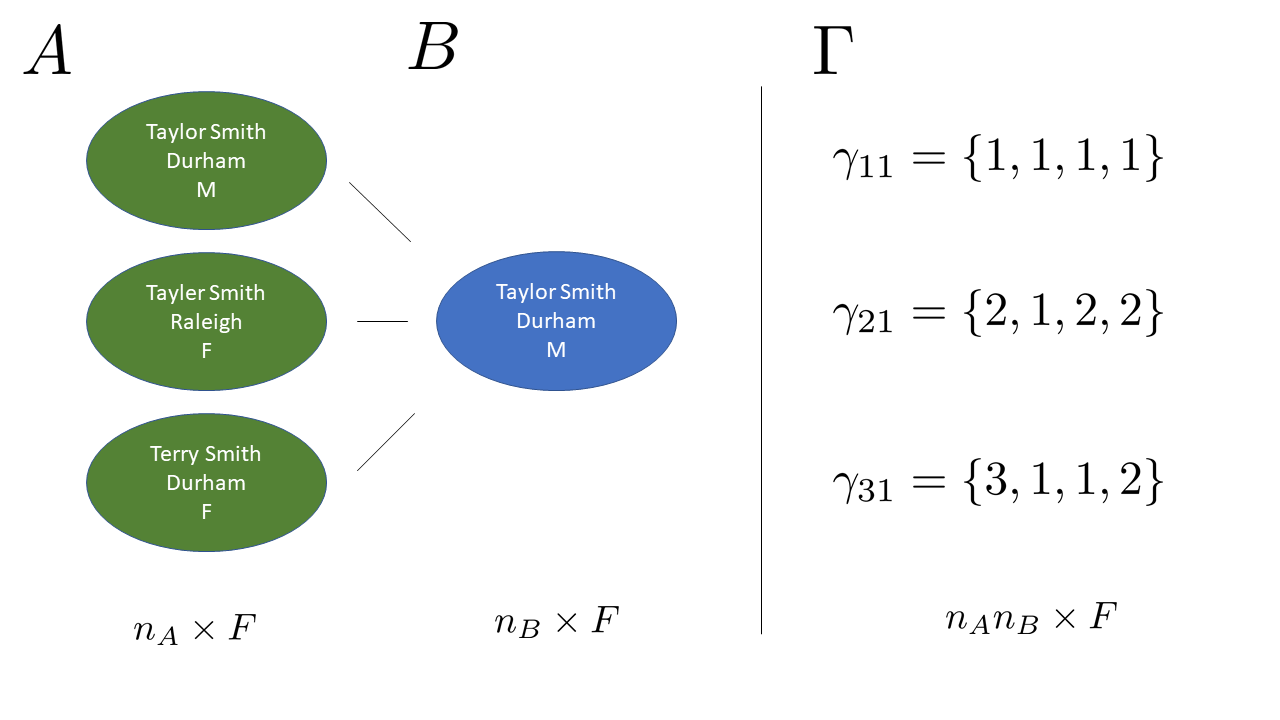
\includegraphics[width = \textwidth, height = .7\textwidth ]{fs_graphic.png}
	\end{frame}

\begin{frame}{Fellegi and Sunter (1969)}
	\begin{columns}
		\begin{column}{0.6\textwidth}
			\includegraphics<1>[width = \textwidth, height = 1.2\textwidth ]{rl_graphics_all/Slide1.png}
			\includegraphics<2->[width = \textwidth, height = 1.2\textwidth ]{rl_graphics_all/Slide2.png}

		\end{column}
		\begin{column}{0.38\textwidth}
			\begin{itemize}
				\item<3-> scalable to large datasets (\texttt{fastlink}, Enamorado et al 2017)
				\item<4-> no transitive closure, requires post-processing
				\pause 
				\item<5-> overmatches, leading to inaccurate parameter estimation
			\end{itemize}

		\end{column}
	\end{columns}
\end{frame}

\begin{frame}{Sadinle (2017) - Beta Record Linkage}
	\begin{columns}
		\begin{column}{0.6\textwidth}
			\includegraphics<1>[width = \textwidth, height = 1.2\textwidth ]{rl_graphics_all/Slide1.png}
			\includegraphics<2>[width = \textwidth, height = 1.2\textwidth ]{rl_graphics_all/Slide3.png}
			\includegraphics<3>[width = \textwidth, height = 1.2\textwidth ]{rl_graphics_all/Slide4.png}
			\includegraphics<4->[width = \textwidth, height = 1.2\textwidth ]{rl_graphics_all/Slide5.png}
			
		\end{column}
		\begin{column}{0.38\textwidth}
			\begin{itemize}
				\item<1-> Beta Record Linkage (\texttt{BRL})
				\pause
				\item<5-> strictly enforces one-to-one matching, no post-processing
				\pause
				\item<6-> high accuracy for linkage and other parameters
				\pause 
				\item<7-> inherently serial, not scalable to large linkage tasks
			\end{itemize}
			
		\end{column}
	\end{columns}
\end{frame}

\begin{frame}{Our Contribution - Fast Beta Linkage}
	\begin{columns}
		\begin{column}{0.6\textwidth}
			\includegraphics<1>[width = \textwidth, height = 1.2\textwidth ]{rl_graphics_all/Slide1.png}
			\includegraphics<2->[width = \textwidth, height = 1.2\textwidth ]{rl_graphics_all/Slide6.png}
			
		\end{column}
		\begin{column}{0.38\textwidth}
			\begin{itemize}
				\item<3-> simple mathematical change, large computational gains
				\item<4-> minimal loss of accuracy for linkage and other parameters, minimal post-processing
			\end{itemize}
			
		\end{column}
	\end{columns}
\end{frame}

\section{Fast Beta Linkage}
\begin{frame}{Notation}
\begin{itemize}
	\item File A with records indexed $i \in \{1, \ldots, n_A\}$ and file B with records $j \in \{1, \ldots, n_B\}$. We use $F$ features for linkage, with $L_f$ possible levels of agreement on feature $f$.
	
	\item $\Gamma \in \mathbb{R}^{n_A n_B \times F}$ matrix of comparison vectors where $\gamma_{ij}^f \in \{1, \ldots, L_f\}$
	
	\item $Z_j = \begin{cases} 
	i,  & \text{if records } i\in A \text{ and } j\in B \text{ match}; \\
	n_A + 1,  & \text{if record } j\in B \text{ has no match in } A; \\
	\end{cases}$
	
	\item $m_{fl} = P\left(\gamma_{ij}^f = l |Z_j = i\right)$
	
	\item $u_{fl} = P\left(\gamma_{ij}^f = l |Z_j \neq i\right)$
	
	\item $\lambda = P(Z_j \leq n_A)$
\end{itemize}
\end{frame}

\begin{frame}{Fast Beta Linkage (fabl)}
	$$P(\Gamma|\mathbf{Z}, \mathbf{m}, \mathbf{u}) = \prod_{j=1}^{n_B}  \prod_{i=1}^{n_A}\left[ \prod_{f=1}^{F}\prod_{l=1}^{L_f} m_{fl}^{I(Z_j = i)}u_{fl}^{I(Z_j \neq i)}\right]^{I(\gamma_{ij}^f = l)}$$
	
	$$\mathbf{m_{f}} \sim \text{Dirichlet}(\alpha_{f1}, \ldots, \alpha_{fL_f})$$
	$$\mathbf{u_{f}} \sim \text{Dirichlet}(\beta_{f1}, \ldots, \beta_{fL_f})$$
	$$Z_j | \lambda =
	\begin{cases} 
	\frac{1}{n_A}\lambda  & z_j \leq n_A; \\
	1-\lambda &  z_j  = n_A + 1 \\
	\end{cases}$$
	$$\lambda \sim \text{Beta}(\alpha_{\lambda}, \beta_{\lambda})$$
	
	Model specification allows for \textbf{parallel/distributed} computing, \textbf{hashing} of comparison vectors, and \textbf{storage efficient indexing (SEI)}
\end{frame}

\begin{frame}{Hashing}
	\begin{itemize}
		\item Recognize there are at most $P = \prod_{f = 1}^F L_f$ unique agreement patterns, regardless of number of records. When $(i,j)$ pair exhibits agreement pattern $p$, say $h(i, j)=p.$
		
		\item Reduce data to sufficient statistics
		\begin{itemize}
		\item $r_{p_j} = \{i \;|\, (i, j) \in h_p\}$
		\item $H_{p_j} = ||r_{p_j}||$
		\item $H_p = \sum_{j} H_{p_j}$
		\end{itemize}
		
		\item Run Gibbs sampler at level of agreement patterns, not record pairs
		\begin{itemize}
		\item Sample the agreement of pattern $h(z_j, j)$, instead of record label $z_j$.
		\item Use number of matches for each pattern to update $m$ and $u$
		\item Back fill record labels at the end through $r_{p_j}$
	\end{itemize}

		\item Reduces computational complexity from $O(n_A \times n_B \times F)$ to $O(P \times n_B \times F)$
	\end{itemize}
\end{frame}

\begin{frame}{Managing Large Data}
	\begin{itemize}
		\item \textbf{Distributed Computing} - Partition data in to chunks $\{A_I\}$ and $\{B_J\}$. Compare records, hash results, compute summary statistics in parallel, and synthesize results.
		
		\item \textbf{Storage Efficient Indexing (SEI)} - Store at most small number $R$ many record labels in each $r_{p_j}$, remove highly unlikely record labels from memory. Proper weights for calculations maintained through summary statistics $\{H_p\}$ and $\{H_{p_j}\}$.
		
		\item Hashing plus SEI can reduce memory requirements by >99%
		\begin{itemize}
			\item Simulation of $20,000 \times 20,000$ linkage task with 4 fields. Naive approach requires 6.4GB of storage for all-to-all comparisons, hashing and SEI requires 90MB.
		\end{itemize}
	\end{itemize}
\end{frame}

\section{Results}

\begin{frame}{Three Simulation Studies}
	\begin{itemize}
		\item We compare \texttt{fabl} against \texttt{BRL} in three simulation studies
		\begin{itemize}
			\item Measure precision and recall on 100 simulated datasets and varying levels of error and duplication across files
			\item Measure speed when both $n_A$ and $n_B$ are increasing
			\item Measure speed when $n_A$ is increasing and $n_B = 500$ is fixed. 
		\end{itemize}
	\end{itemize}
\end{frame}

	\begin{frame}{Accuracy Simulation}
	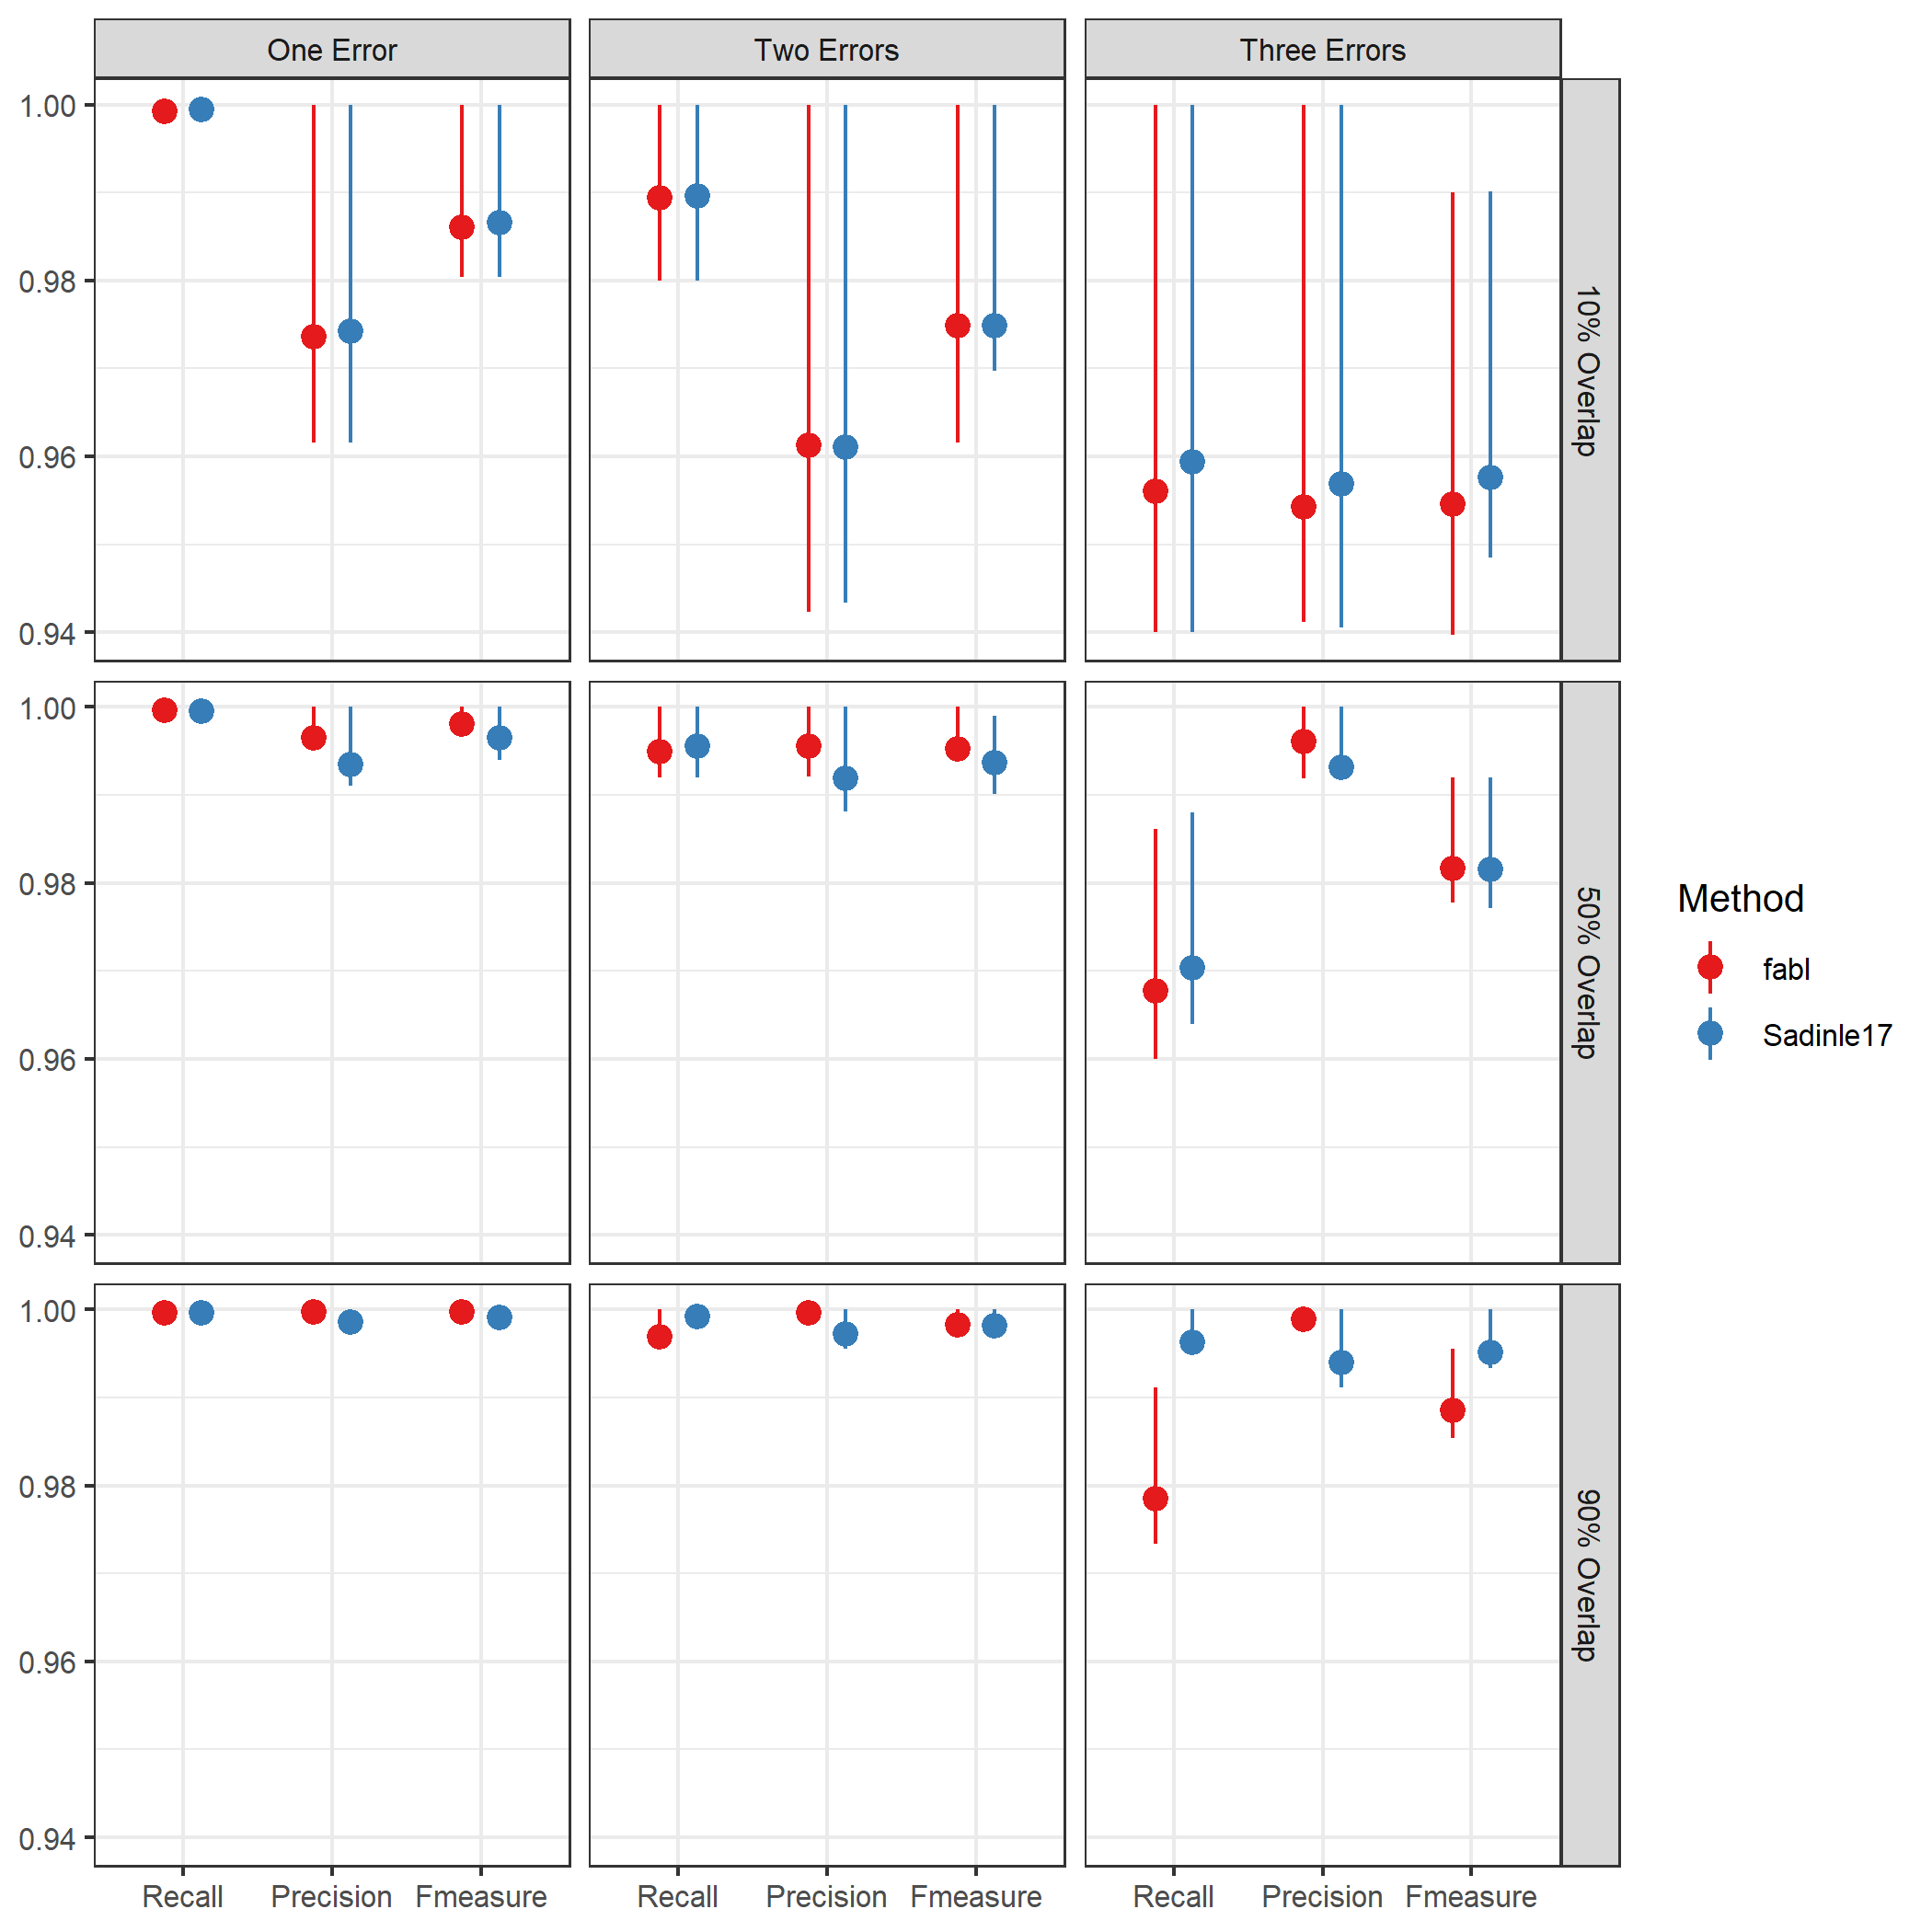
\includegraphics[width = \textwidth, height = .7\textwidth ]{../notes/figures/sadinle_sim_plot.png}
\end{frame}

	\begin{frame}{Speed Simulation 1}
	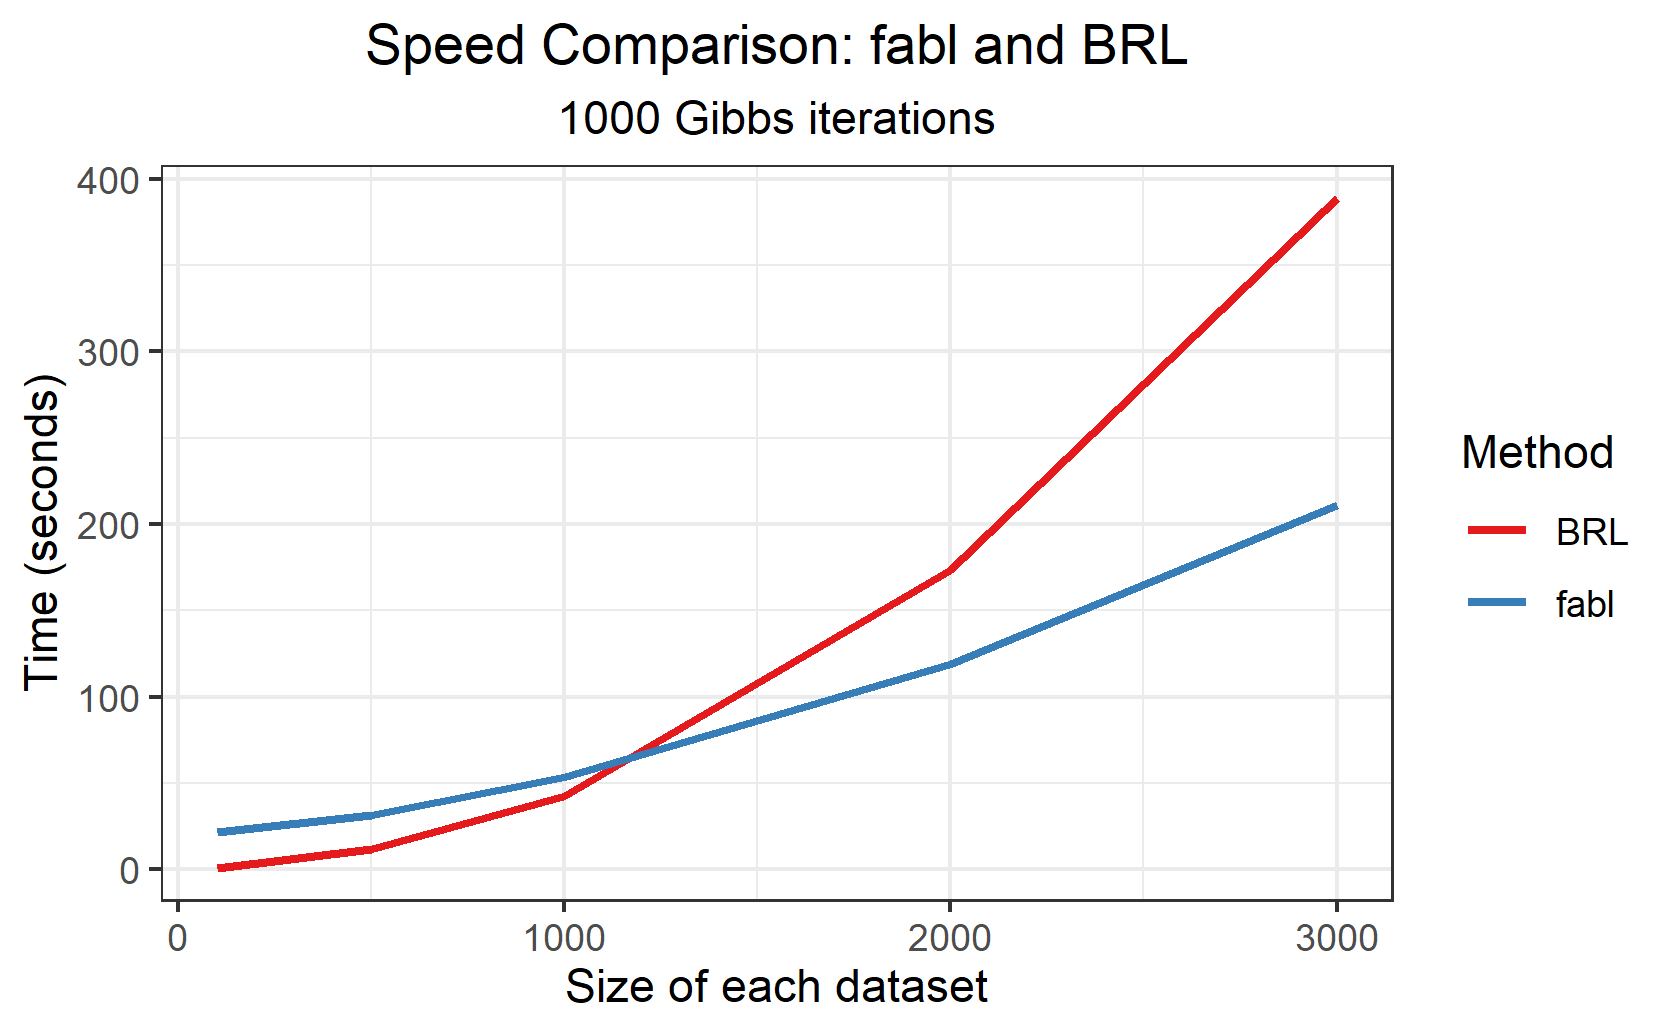
\includegraphics[width = \textwidth, height = .7\textwidth ]{../notes/figures/sadinle_speed_plot2.png}
\end{frame}

	\begin{frame}{Speed Simulation 2}
	
\includegraphics[width = \textwidth, height = .7\textwidth ]{../notes/figures/speed_plot_fixed_nB.png}
\end{frame}

\begin{frame}{Extensions and Directions}
	\begin{itemize}
	\item Linkage in the face of duplicates within datasets
	
	\item Models that allow reliability of information to differ by subgroup in the data
	
	\item Linkage over blocked data (allows for much larger linkage tasks)
	\end{itemize}
\end{frame}

\end{document}